\chapter{Bausteinsicht}
In diesem Kapitel zeigen wir den Aufbau des Condition Monitoring Systems. Es werden dabei die grundlegenden Pakete, Programmstrukturen und Komponenten beschrieben.
\section{Ebene 1}
Die Bausteine der ersten Ebene sind die zu implementierenden Einheiten. Die verschiedenen Module enthalten unterschiedliche Architekturstile, wordurch unser Gesamtsystem eine heterogene Softwarearchitektur aufweist. Jedes Modul verantwortet einen Teil der Gesamtfunktionalität. Anhand dieser werden die folgenden Ebenen um weitere Einheiten erweitert. Die folgende Grafik gibt einen ersten Überblick über das System.
\begin{figure}[h]
	\centering
	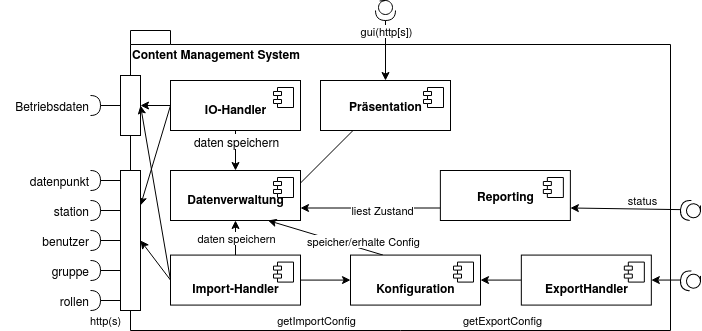
\includegraphics[width=1.0\textwidth]{Graphics/bausteinansicht_ebene_1.png}
	\caption{Bausteinsicht Level 1}
	\label{fig:bausteinsichtlvl1}
\end{figure}
Die Module IO-Handler und Datenverwaltung sind hauptverantwortlich für das Architekturziel hohe Performance.
Das Architekturziel der Verfügbarkeit wird von den Komponenten Reporting und ExportHandler gewährleistet. 
Das PräsentationManager-Modul verantwortet, dass das Architekturziel der Benutzerfreundlichkeit eingehalten wird.
Die folgenden Abschnitte beschreiben die in der Abbildung dargestellten Einheiten ausführlicher.
\clearpage
\subsection{IO-Handler}
\begin{table}[th]
	\begin{tabularx}{\textwidth}{p{5cm} X}
		\hline
		 Zweck/Verantwortlichkeit & Das Modul nimmt über Außenschnittstellen die Daten von Fremdsystemen entgegen. \\
		 \hline
		 Schnittstellen &  Eingang von Betriebsdaten(csv, json, binär). Nutzt Funktionen aus der Datenverwaltung \\
		 \hline
	\end{tabularx} 
	\caption{IO-Handler}
	\label{tab:IO-Handler}
\end{table}

\subsection{Präsentation Manager}
\begin{table}[th]
	\begin{tabularx}{\textwidth}{X X}
		\hline
		Zweck/Verantwortlichkeit & Anzeigeoberflächenverwaltung für Benutzer \\
		\hline
		Schnittstellen & Nutzt Daten und Funktionen aus der Datenverwaltung\\
		\hline
	\end{tabularx} 
	\caption{Präsentation Manager}
	\label{tab:Präsentation Manager}
\end{table}

\subsection{Datenverwaltung}
\begin{table}[th]
	\begin{tabularx}{\textwidth}{X X}
		\hline
		Zweck/Verantwortlichkeit & Verwaltet sämtliche Daten und beinhaltet Funktionsblöcke die Verwaltungsoperation Lesen, Schreiben und Löschen für die Daten Datenpunkt, Station, Benutzer, Gruppe, Rollen, Report und Regeln bereitstellen. \\
		\hline
		Schnittstellen & Erhält Daten von dem IO-Handler und stellt diese durch Funktionen im Präsentation Manager bereit\\
		\hline
	\end{tabularx} 
	\caption{Datenverwaltung}
	\label{Datenverwaltung}
\end{table}
\clearpage
\subsection{Reporting}
\begin{table}[th]
	\begin{tabularx}{\textwidth}{p{5cm} X}
		\hline
		Zweck/Verantwortlichkeit & Erstellt Backupdaten und liefert über die Aussenschnittstellen Berichtdaten \\
		\hline
		Schnittstellen & Nutzt die Funktionen der Datenverwaltung um Reports zu erstellen\\
		\hline
	\end{tabularx} 
	\caption{Reporting}
	\label{tab:Reporting}
\end{table}

\subsection{Export-Handler}
\begin{table}[th]
	\begin{tabularx}{\textwidth}{p{5cm} X}
		\hline
		Zweck/Verantwortlichkeit & Liefert über Außenschnittstellen Übersichtsdaten \\
		\hline
		Schnittstellen & Übersichtsdaten(PDF, CSV, JSON) und nutzt dabei Methoden aus der Dateiverwaltung\\
		\hline
	\end{tabularx} 
	\caption{Export-Handler}
	\label{tab:ExportHandler}
\end{table}

\section{Ebene 2}
Die Darstellung der Bausteine der zweiten Ebene zeigt die Hauptbausteine der einzelnen Module.
\begin{figure}[h]
	\centering
	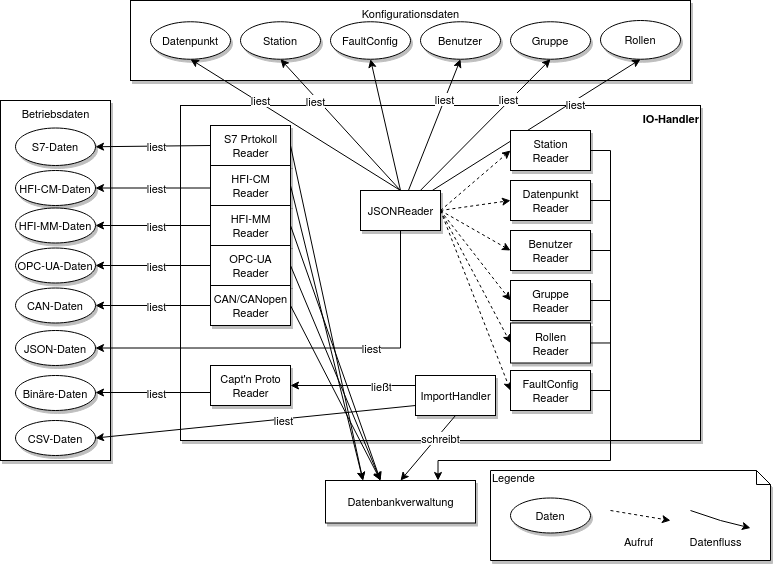
\includegraphics[width=1\textwidth]{Graphics/bausteinansicht_ebene_2_IO-Modul.png}
	\caption{Bausteinsicht Level 2 IO-Handler}
	\label{fig:bausteinsichtlvl2_modulIO}
\end{figure}                 

\begin{table}[t]
	\begin{tabularx}{\textwidth}{|p{5cm}| X|}
		\hline
		Baustein & Beschreibung\\
		\hline
		Readerkomponenten & Jede Readerkomponente ist für das einlesen einer bestimmten Protokollart zuständig. Der JSONReader unterteilt sich jeweils noch für die einzelnen Konfigurationsdaten sodass jede Dartenart gelesen werden kann. Jede dieser Daten werden in diese Komponenten deserialisiert. Jeder Reader leitet sein Ergebniss an die Datenbankverwaltung weiter. \\
		\hline
		Import Handler &  Nimmt über die Außenschnittstellen alle Daten im CSV- und binärformat auf und sendet diese an die Datenbankverwaltung\\
		\hline
	\end{tabularx} 
	\caption{Beschreibung Bausteine IO-Handler}	\label{tab:IOHandlerBeschreibung}
\end{table}

\begin{figure}[h]
\centering
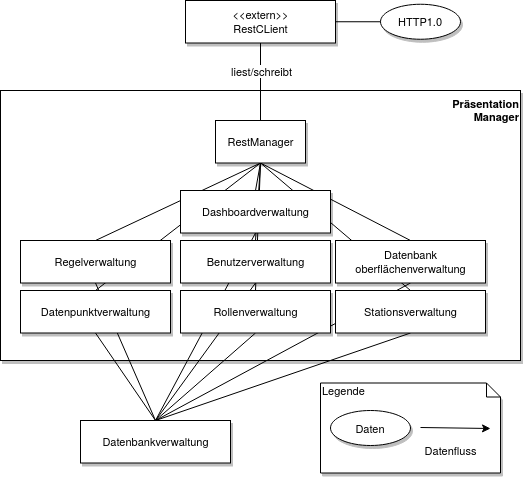
\includegraphics[width=1\textwidth]{Graphics/bausteinansicht_ebene_2_PrasentationManager.png}
\caption{Bausteinsicht Level 2 Pr\"asentation Manager}
\label{fig:bausteinsichtlvl2__PrasentationManager}
\end{figure}                 

\begin{table}[th]
	\begin{tabularx}{\textwidth}{|p{5cm}|X|}
		\hline
		Baustein & Beschreibung\\
		\hline
		Verwaltungskomponenten & Jede Verwaltungskomponente stellt ViewModel-Klassen mit Data Binding und zugehörigen Views zur Verfügung. Die den Views und ViewModels zugehörigen Models und Daten, sind die Relationen und Schemen aus der Konfigurationsdatenbank. \\
		\hline
		RestManager &  Der RestManager stellt das System nach außen hin dar. Er verwaltet GET, POST und DELETE anfragen für jeden Endpunkt. Die Endpunkte werden durch die Verwaltungskomonenten dargestellt. An diese übergibt der RestManager die Befehle bei entsprechenden HTTP-Reuquests.\\
		\hline
	\end{tabularx} 
	\caption{Beschreibung Baustein PrasentationManager}	\label{tab:Representation}
\end{table}

\begin{figure}
	\centering
	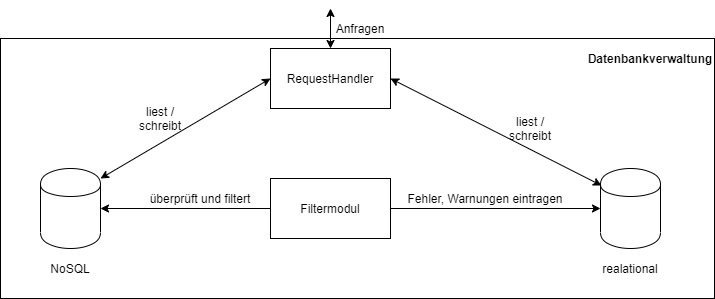
\includegraphics[width=1\textwidth]{Graphics/datenbankverwaltung.png}
	\caption{Datenbankverwaltung}
	\label{fig:datenbankverwaltung}
\end{figure}

\begin{table}[th]
	\begin{tabularx}{\textwidth}{|p{5cm}| X|}
		\hline
		Baustein & Beschreibung\\
		\hline
		RequestHandler & Verarbeitet alle Anfragen und entscheidet, welche Anfrage zu welcher Datenbank weitergeleitet werden muss. Die Ergebnisse der Datenbanken werden wiederum an den Empfänger zurückgesendet. \\
		\hline
		Filtermodul & Überprüft eigenständig alle Daten in der NoSQL Datenbank auf Korrektheit und bei Auffälligkeiten werden diese in die relationale Datenbank abgelegt oder direkt gelöscht.\\
		\hline
		NoSQL & Hypertable-Datenbank für Maschinen- und Sensordaten\\
		\hline
		realtional & SQLite-Datenbank für User- und andere Daten\\
		\hline
	\end{tabularx} 
	\caption{Beschreibung Baustein Datenbankverwaltung}
	\label{tab:Datenbankverwaltung}
\end{table}